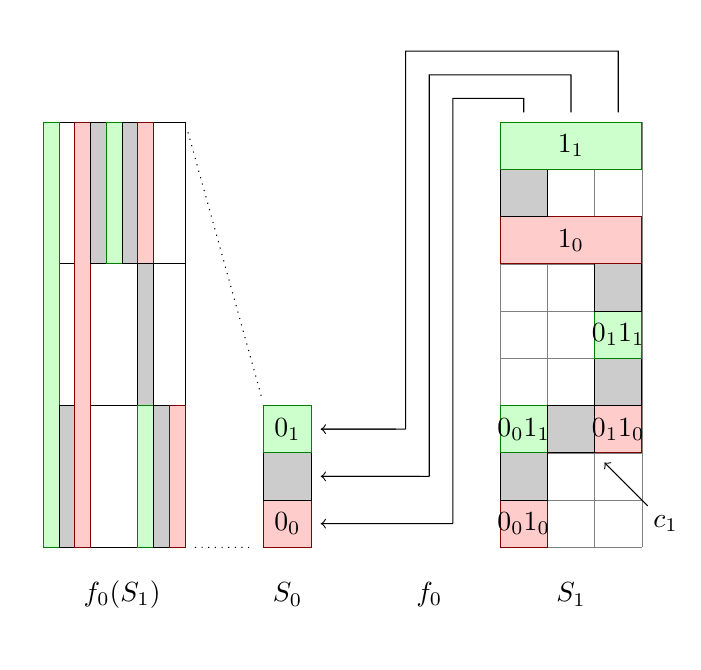
\begin{tikzpicture}[xscale=0.6,yscale=0.6]
\useasboundingbox  rectangle (13.6653,12.9987);

% S_0

\draw[fill=red!20, draw=red!50!black]  (5,3) rectangle (6,2);
\draw[fill=black!20]  (5,4) rectangle (6,3);
\draw[fill=green!20, draw=green!50!black]  (5,5) node (v23) {} rectangle (6,4);

\node at (5.5,4.5) {$0_1$};
\node at (5.5,2.5) {$0_0$};

\node at (5.5,1) {\normalsize $S_0$};


%  S_1

\draw[step=1cm,gray,very thin] (10,2) grid (13,11);

\draw[fill=red!20, draw=red!50!black]  (10,3) rectangle (11,2);
\draw[fill=black!20]  (10,4) rectangle (11,3);
\draw[fill=green!20, draw=green!50!black]  (10,5) rectangle (11,4);

\draw[fill=red!20!white, draw=red!50!black]  (12,5) rectangle (13,4);
\draw[fill=white!80!black]  (12,6) rectangle (13,5);
\draw[fill=green!20!white, draw=green!50!black]  (12,7) rectangle (13,6);

\draw[fill=white!80!black]  (11,5) rectangle (12,4) node (v2) {};

\draw[fill=white!80!black]  (12,8) rectangle (13,7);
\draw[fill=red!20!white, draw=red!50!black]  (10,9) rectangle (13,8);
\draw[fill=white!80!black]  (10,10) rectangle (11,9);
\draw[fill=green!20!white, draw=green!50!black]  (10,11) rectangle (13,10);

\node at (11.5,10.5) {$1_1$};
\node at (11.5,8.5) {$1_0$};
\node at (12.5,6.5) {$0_11_1$};
\node at (12.5,4.5) {$0_11_0$};
\node at (10.5,4.5) {$0_01_1$};
\node at (10.5,2.5) {$0_01_0$};

\node at (11.5,1) {\normalsize $S_1$};


% c_1

\node (v1) at (13.5,2.5) {\normalsize $c_1$};
\draw [->] (v1) edge (v2);


% f_0

\node (v3) at (10.5,11) {};
\node (v7) at (11.5,11) {};
\node (v12) at (12.5,11) {};
\node (v16) at (6,4.5) {};
\node (v11) at (6,3.5) {};
\node (v17) at (6,2.5) {};
\node (v4) at (10.5,11.5) {};
\node (v8) at (11.5,12) {};
\node (v13) at (12.5,12.5) {};
\node (v5) at (9,11.5) {};
\node (v9) at (8.5,12) {};
\node (v14) at (8,12.5) {};
\node (v15) at (8,4.5) {};
\node (v10) at (8.5,3.5) {};
\node (v6) at (9,2.5) {};

\draw [-](v3) -- (v4.center) -- (v5.center) -- (v6.center);
\draw [-](v7) -- (v8.center) -- (v9.center) -- (v10.center);
\draw [-](v12) -- (v13.center) -- (v14.center) -- (v15.center);
\draw [-] (v15.center) edge (v16);
\draw [->] (v15) edge (v16);
\draw [-] (v10.center) edge (v11);
\draw [->] (v10) edge (v11);
\draw [-] (v6.center) edge (v17);
\draw [->] (v6) edge (v17);

\node at (8.5,1) {\normalsize $f_0$};


% f_0(S_1)

\draw (0.3334,10.9989) node (v18) {} rectangle (3.3334,7.9989);
\draw (0.3334,7.9989) rectangle (3.3334,4.9989);
\draw (0.3334,4.9989) rectangle (3.3334,1.9989) node (v22) {};

\draw [fill=green!20!white, draw=green!50!black]  (v18) rectangle (0.6654,1.9987);
\draw [fill=white!80!black] (0.6654,4.9984) rectangle (0.9987,1.9987) node (v19) {};
\draw [fill=red!20, draw=red!50!black]  (v19) rectangle (1.332,10.9978) node (v20) {};
\draw [fill=white!80!black] (v20) rectangle (1.6653,7.9981);
\draw [fill=green!20!white, draw=green!50!black]  (1.6653,10.9978) rectangle (1.9986,7.9981);
\draw [fill=white!80!black] (1.9986,10.9978) rectangle (2.3319,7.9981);
\draw [fill=red!20, draw=red!50!black]  (2.3319,10.9978) rectangle (2.6652,7.9981);
\draw [fill=white!80!black] (2.3319,7.9981) rectangle (2.6652,4.9984) node (v21) {};
\draw [fill=green!20!white, draw=green!50!black]  (2.3319,4.9984) rectangle (2.6652,1.9987);
\draw [fill=white!80!black] (v21) rectangle (2.9985,1.9987);
\draw [fill=red!20, draw=red!50!black]  (2.9985,4.9984) rectangle (v22);

\node at (2,1) {\normalsize $f_0(S_1)$};

\node (v24) at (3.333,10.9989) {};
\node (v25) at (4.9995,1.9998) {};
\node (v26) at (5.9994,4.9995) {};
\draw [-,dotted] (v23) edge (v24);
\draw [-,dotted] (v22) edge (v25);
\node at (-1.3332,-4.3329) {};
\end{tikzpicture}